%!TEX encoding = UTF-8 Unicode
\documentclass[ % options,
    a4paper,    % papersize
%    cjk,       % for cjk-ko
%    usedotemph,% for cjk-ko's \dotemph
    amsmath,    % load amsmath.sty to typeset math materials
    itemph,     % to disable gremph default (xe/lua)
%    footnote,  % korean style footnote
%    chapter,   % to use \chapter
]{oblivoir}     % xoblivoir and oblivoir are identical.

\ifPDFTeX       % latex, pdflatex
%    \usepackage{newtxtext}    % Latin fonts
\else\ifLuaOrXeTeX   % xelatex or lualatex
%  \setmainfont[Ligatures=TeX]{TeX Gyre Termes}   %% Latin fonts
  \defaultfontfeatures{Ligatures=TeX}
  \setkormainfont(* ExtraBold)(*){NanumGothic}(* Bold)(*){HCR Batang LVT}
  \setkorsansfont{NanumGothic}
  \setkormonofont[Scale=.95]{NanumGothic}
\fi\fi

\usepackage{kotex-logo}
\usepackage{hyperref}
\usepackage{amsthm}
\usepackage{tcolorbox}
\usepackage{geometry}
\usepackage{graphicx}
\newtheorem{thm}{Theorem}[section]
\theoremstyle{definition}
\newtheorem{dfn}{Definition}[section]
\theoremstyle{remark}
\newtheorem{note}{Note}[section]
\newtheorem{insight}{Insight}[section]
\theoremstyle{plain}
\newtheorem{lem}[thm]{Lemma}

% 단락 변경시 들여쓰기를 0으로 만듦 (한글이 이게 이쁘다)
\setlength{\parindent}{0em}
% 단락 간의 간격을 1로 만듬
\setlength{\parskip}{1em}
% brown 색상 정의
\definecolor{brown1}{RGB}{128,64,0}
% subsubsection이 번호를 갖게 함
\setcounter{secnumdepth}{3}


\begin{document}

\pagestyle{headings}

\title{모바일 RPG에서 서버 시뮬레이션 분산과 플레이 검증}
\author{Darkface}
\date{\today}
\maketitle

\begin{abstract}
\end{abstract}

\tableofcontents

\section{개요}

모바일이 주력 플래폼으로 떠오른 지 이미 오래 되었다. 웹젠의 주력 게임은 아직 RPG이고
RPG 게임들을 만들고 있다. RPG 게임들은 캐릭터의 능력치, 아이템과 장비에 따른 능력치 상승을 포함하여
전체적으로 능력치의 상승을 추가되는 공간과 관계 속에서 즐기는 게임이다.

따라서, 능력치을 올리는 것이 게임의 핵심 목표이며 여기에 대부분의 시간을 할당하게 된다.
초기 모바일 RPG들은 거래가 없고 빠른 액션감 대신 시뮬레이션과 그래픽적인 표현의 만족을 주로 제공했다.
이런 게임들은 어뷰징이나 크랙(해킹)에서 비교적 피해가 적었다. 반면에 다크어벤저 I, II는 액션성과
중국 사용자들이 서비스 초기부터 몰려오면서 게임 머니 생성을 포함하여 상당히 많은 피해를 본 경우이다.

멀티 플레이를 제공하는 게임들은 사용자들이 인지하는 경쟁의 정도가 높아질 수 밖에 없어
해킹이 좀 더 광범위하게 퍼질 가능성이 높으며 초기부터 멀티 플레이 대전이 있었던 다크어벤저도
이런 경우에 포함된다고 본다.

다양한 원인이 있지만 일반적으로 멀티플레이를 지원하는 게임들이 늘어나고 게임 플레이 타임이 증가하고
유료화 결제율도 증가하고 있으며 블루스택과 같이 PC에서 돌아가는 VM 기반의 에뮬레이터의 확산으로
해킹은 점점 더 늘어날 가능성이 높아 보인다.

\section{모바일 게임 개발 특성}

\subsection{작은 규모}
모바일 게임은 작은 규모로 개발되고 있고 NC 스타일의 대규모 물량을 투자하는 방식의 게임들이
시장을 장악하는 상황으로 넘어가지 않는다면 이런 경향은 지속될 가능성이 높다. 사용자들의 선택이나
시장의 트렌드에 따라 변화될 여지는 있으나 짧은 시간 플레이하고 이를 연속적으로 이어가는 방식의 게임들이
주류를 차지하고 있어 어떻게 변화할 지 판단하기 어렵다.

\begin{tcolorbox}[colback=green!5,colframe=green!40!black,title=인력 규모]
\begin{insight}[인력규모]
  당분간 적은 인력을 유지한 코어 팀과 아웃소싱 중심으로 개발이 지속될 것이다.
\end{insight}
\end{tcolorbox}

\subsection{빠른 변화, 빠른 개발}
모바일 시장은 빠르게 변화하고 있으며 지역별 특화 현상도 심화되고 있는 것으로 보인다. 중국, 한국 중심으로
RPG 게임등이 현재 시장을 주도하고 있으나 한국도 전략 게임, 라이트 RPG들이 선전하고 있으며 모두의 마블처럼
고포류 게임들도 상위권으로 올라올 수 있는 동력이 있다.

런류 게임들이 한 때 엄청 개발되던 시기가 있었던 것을 돌아보면 변화를 절감할 수 있고
예전의 플래포머들이나 유명 IP 기반의 게임들, 또는 참신한 통합과 변화를 시도한 게임들이
일정 시기 주류 게임들로 부상할 수 있다.

변화가 빠른 상황은 빠른 개발을 할 수 밖에 없도록 만들고 있다. 따라서, 모바일 게임 개발에서 빠른 개발은 중요하다.
아니면 매우 창조적인 게임을 긴 시간 공을 들여 개발할 수는 있는데 자본 수익율이나 기업의 존속을 위해서는
적은 팀을 유지할 수 밖에 없다.

\begin{tcolorbox}[colback=green!5,colframe=green!40!black,title=빠른 개발]
\begin{insight}[빠른 개발]
  변화가 일어나는 모바일 시장에서 성공하기 위해서는 빠른 개발이 필수적이다.
\end{insight}
\end{tcolorbox}

\subsection{백엔드 아키텍처의 변화}
초기 모바일 RPG들은 멀티 플레이를 지원하지 않았고 Zinga에서 시작된 웹 서비스와 유사한
웹 기반, NoSQL / RDBMS 혼합 모델로 클라이언트 주도형 게임 플레이 구현이 주된 아키텍처였다.
그래서, 한 때 채팅을 지원하는 게임이 별반 없었고 실시간 동시 플레이를 제공하는 게임도 적었다.

이후 P2P를 릴레이를 통해 제공하는 다크어벤저와 같은 게임들이 출시되었고
멀티플레이가 되는 것만으로도 사용자들 반응이 일부 있었으나
모바일에서 멀티플레이 자체는 영웅의 군단이나 우리의 뮤 오리진이 본격적인 MMO 기능을 가져오기 전까지는
미미한 수준이었다.

뮤 오리진은 웹 게임 전문 개발사에서 개발한 게임으로 서버가 게임플레이를 주도하는 방식이며
이동, 피격 판정, 드랍, 루팅, 그 외 컨텐츠를 서버를 통해서 처리하는 것으로 보인다.
웹 게임 개발사 답게 서버와 통신은 IIS의 웹 소켓 기능을 사용하고 소켓을 유지한 상태로
별도의 시뮬레이션 프레세스와 연결하여 처리하는 것으로 보인다.

\begin{figure}[h!]
\centering
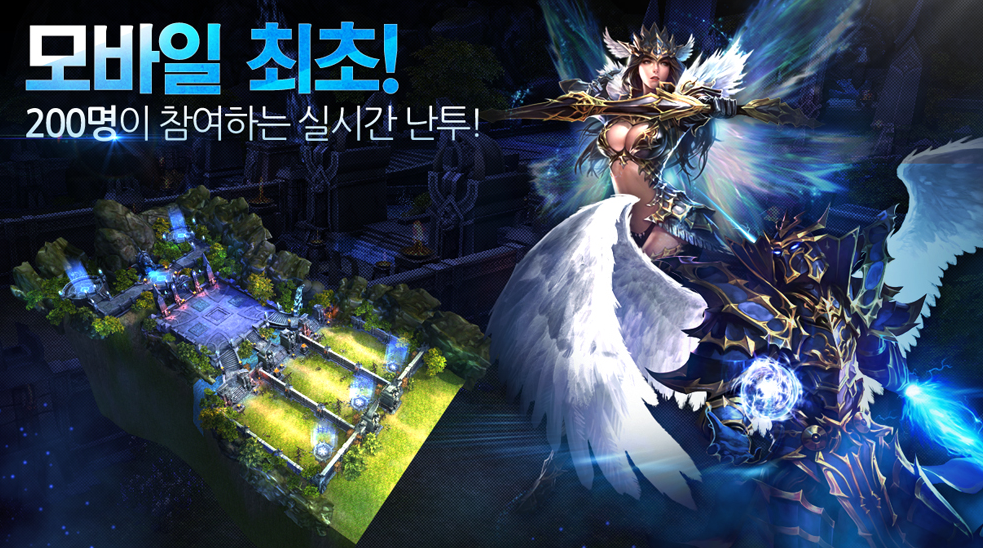
\includegraphics[scale=0.5]{mu_origin.png}
\caption{MU Origin - 공성전 광고}
\label{fig:mu_origin}
\end{figure}

뮤 오리진은 담벼락 등의 장애물이 있어도 뚫고 공격할 수 있으며 대부분 평평한 바닥 구조를 갖고 있고
판정도 2D 범위 판정으로 보이며 몬스터들이 길을 찾는 방식은 클라이언트 도움을 받는 구조일 수 있다.

뮤 오리진의 성공 이후 많은 MMORPG들이 모바일로 출시될 것으로 보이며
RPG에서 멀티 플레이가 매우 중요한 요소 중의 하나인 게임들이 점점 더 많아질 것으로 보인다.

이는 데이터 저장과 전달 중심의 서버에서 게임 플레이를 중계하고 검증을 하는 서버 기능이
필요해 지는 것을 의미하며 MMORPG의 구성 요소 중 적은 규모의 팀이 빠르게 개발할 수 있는
한계 안에서 서버 시뮬레이션과 동기화 기능이 추가되는 것을 의미한다.

\begin{tcolorbox}[colback=green!5,colframe=green!40!black,title=서버 아키텍처의 변화]
\begin{insight}[서버 아키텍처의 변화]
  모바일 게임 서버는 동기화와 시뮬레이션 기능을 갖게 될 것이다. 그 수준은 적은 규모, 빠른 개발이
  가능한 범위로 제한될 것이다.
\end{insight}
\end{tcolorbox}

\section{MORPG의 동기화}

\subsection{MORPG만 고려}
MORPG는 MMORPG와 다른 방식의 동기화를 갖고 있다. 작은 규모의 개발이 필수적인 모바일 개발에서
MMORPG와 같이 완전히 서버에서 개발하는 방식은 상당한 무리가 있다. 게임 내 오브젝트들 (또는 엔티티들)을
하나 하나 움직이고 클라이언트와 동기화 하고 모든 판정을 하는 MMORPG의 방식은 서버 개발 기간이
길 수 밖에 없기 때문에 직접 고려 대상이 아니다.

또 C9 모바일 개발을 위한 지원 작업의 일부로 진행하고 있기 때문에 빠른 액션성을 갖는 게임의 경우
서버와 협업하는 수준이 높을 경우 피드백을 빠르게 하기 위한 추가적인 트릭들이 필요하기 때문에
난이도가 급격하게 올라 갈 수 있다.

따라서, 여기서는 MORPG만을 대상으로 한다.

\begin{tcolorbox}[colback=green!5,colframe=green!40!black,title=MORPG]
\begin{dfn}[MORPG]
MORPG는 Multiplayer Online Role Playing Game의 약자로 요청에 의해 생성되는 인스턴스 공간에서
다수(1--16명 내외)의 플레이가 함께 플레이 할 수 있는 게임의 형태를 말한다.
\end{dfn}
\end{tcolorbox}

\subsection{동기화 목표}
게임의 상태를 클라이언트(들)와 서버가 정보 전달을 통해 일치 시키는 과정이 동기화이며 동기화를 하는 목표는
다음과 같다:
\begin{tcolorbox}[colback=green!5,colframe=green!40!black,title=동기화 목표]
\begin{itemize}
  \item{상태 일치} -- 다른 클라이언트와 게임 상태를 맞추기 위해 서버와 정보를 교환하고
  서버는 다른 클라이언트에게 전달한다. 각 게임 시뮬레이션 주체(클라이언트, 서버)는 게임 상태를 업데이트 한다.
  \item{판정과 보상} -- 요청된 행동에 대한 결과를 계산하고 게임에 반영한다
  \item{검증} -- 요청된 행동이 적합한 지 판단하고 오류가 있을 경우 정정하거나 통보한다
\end{itemize}
\end{tcolorbox}

개별 내용은 방대하며 게임마다 다르고 선택할 수 있는 방벋도 다양하다. 각 목표 영역별 수준을 결정하는 것이 중요하다.

\begin{tcolorbox}[colback=green!5,colframe=brown1!40!black,title=제외 항목]
\begin{note}
  요청과 응답 형식으로 정보를 조회하거나 저장하는 처리는 제외한다. 이 부분도 동기화로 생각할 수 있으나
  모든 게임에서 필수적으로 포함되는 부분이고 서버에서 기본으로 구현되므로 동기화 관련된 이슈는 없다.
  오히려 서버의 응답 속도를 유지하면서 확장하는 것이 더 중요하다. 이 부분은 NoSQL / NewSQL 관련 진행에서
  정리해 나갈 예정이다. 우리의 경우 마의에서 DB 쪽 성능 이슈로 인해 서비스를 제대로 제공하지 못한 경험이 있어
  방향 정리가 필요하다.
\end{note}
\end{tcolorbox}

\subsection{상태일치}

\subsubsection{게임 플레이 구성 요소}

MORPG의 게임 플레이를 구성하는 요소는 다음과 같다.
\begin{tcolorbox}[colback=green!5,colframe=green!40!black,title=게임 플레이 구성 요소]
\begin{itemize}
  \item{게임 배경} -- 이동과 충돌이 일어나는 공간
  \item{게임 오브젝트} -- 플레이어, Npc, 각종 트리거, 동적인 장애물들
\end{itemize}
\end{tcolorbox}

\begin{figure}[h!]
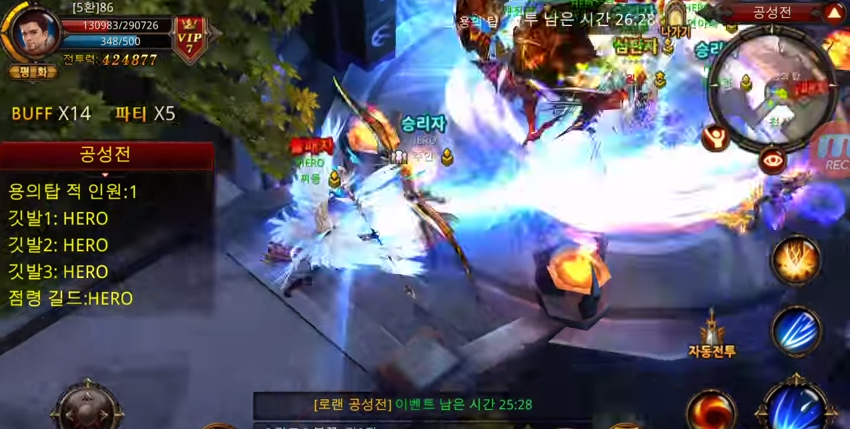
\includegraphics[scale=0.6]{mu_origin_battle.png}
\caption{MU Origin - 전투 : 배경과 플레이어로 구성}
\label{fig:mu_origin_battle}
\end{figure}

이펙트, 트레일, 각종 그래픽적인 표현은 게임 플레이에 영향을 미치지 않는다.
충돌하는 이펙트와 같은 경우 게임에 따라 오브젝트가 될 수도 있다.
애니메이션은 플레이어, Npc와 같은 캐릭터의 경우 게임 시뮬레이션 결과에 영향을 미칠 수 있다.

각종 정적으로 구성된 기획 데이터들은 게임 오브젝트들을 통해서만 발현되므로 직접적인 요소에서 제외한다.

\subsubsection{게임 상태 구성 요소}

게임 오브젝트들은 공간과 관련된 값과 상태를 갖는다.

\begin{tcolorbox}[colback=green!5,colframe=green!40!black,title=공간 요소]
\begin{itemize}
  \item{현재 위치} -- 놓여진 장소이다.
  \item{현재 회전값} -- 방향. 보통은 서 있는 상태이나 장애물이거나 발사체라면 3개 축이 다 필요하다.
  \item{목표 위치} -- 이동할 경우 목표 지점
  \item{속도 / 가속도 / 충격량} -- 물리적인 시뮬레이션이 있을 경우
  \item{중력 등 다른 물리량} -- 물리적인 시뮬레이션이 있을 경우 변화될 수 있다.
\end{itemize}
\end{tcolorbox}

\begin{tcolorbox}[colback=green!5,colframe=green!40!black,title=상태 요소]
\begin{itemize}
  \item{중요 상태} -- FSM을 구성할 때 추가하는 상태들. Idle, Move, Casting, Jump, Looting, Die 등
  \item{부가 상태} -- 버프, 디버프, 물약 효과 등등
\end{itemize}
\end{tcolorbox}

\subsubsection{게임 상태 변경 원인}



\subsubsection{동기화 접근 방식}


\subsection{판정과 보상}


\subsection{검증}


\subsection{방향의 결정}


\section{Warp.Unity - RPG 서버 검증을 위한 필수 요소}







\end{document}
